\documentclass[aspectratio=169]{beamer}
\usetheme{Madrid}
\usecolortheme{default}
\usepackage{booktabs,amsmath}
\graphicspath{{figs/}}
% Auto-generated by exec13_230_fixed_scale.py
% Source: exec13_230_core_resolution.csv — do not edit manually
% EJ-230 (OPSC-106): TAU_D = 1.5 ns (NOT 1.8 ns of EJ-204)
% No EXEC_12-EJ230 reference exists; ExecTwelveRef macros omitted.

\newcommand{\ejtauD}{1.5}
\newcommand{\ejYield}{9700}

% Run 1 x=-690 mm ID 16
\newcommand{\coreRunOneRMSps}{44.00}
\newcommand{\coreRunOneSigCore}{29.67}
\newcommand{\coreRunOneSigCoreErr}{5.98}
\newcommand{\coreRunOneChiNdf}{33.36}
\newcommand{\coreRunOneIQR}{2.13}
\newcommand{\coreRunOneMAD}{1.95}
\newcommand{\coreRunOneCoreFrac}{0.90}
\newcommand{\coreRunOneTailFrac}{0.10}
\newcommand{\coreRunOneTailPct}{10}
\newcommand{\coreRunOneSigEx}{7.77}
\newcommand{\coreRunOneSigStat}{9.41}
\newcommand{\coreRunOneNearestID}{16}

% Run 3 x=-400 mm ID 31
\newcommand{\coreRunThreeRMSps}{50.63}
\newcommand{\coreRunThreeSigCore}{2.02}
\newcommand{\coreRunThreeSigCoreErr}{0.04}
\newcommand{\coreRunThreeChiNdf}{2.35}
\newcommand{\coreRunThreeIQR}{4.32}
\newcommand{\coreRunThreeMAD}{3.14}
\newcommand{\coreRunThreeCoreFrac}{0.76}
\newcommand{\coreRunThreeTailFrac}{0.24}
\newcommand{\coreRunThreeTailPct}{24}
\newcommand{\coreRunThreeSigEx}{11.37}
\newcommand{\coreRunThreeSigStat}{8.17}
\newcommand{\coreRunThreeNearestID}{31}

% Run 4 x=+0 mm ID 50
\newcommand{\coreRunFourRMSps}{53.61}
\newcommand{\coreRunFourSigCore}{2.49}
\newcommand{\coreRunFourSigCoreErr}{0.04}
\newcommand{\coreRunFourChiNdf}{3.61}
\newcommand{\coreRunFourIQR}{21.72}
\newcommand{\coreRunFourMAD}{4.61}
\newcommand{\coreRunFourCoreFrac}{0.73}
\newcommand{\coreRunFourTailFrac}{0.27}
\newcommand{\coreRunFourTailPct}{27}
\newcommand{\coreRunFourSigEx}{9.55}
\newcommand{\coreRunFourSigStat}{8.20}
\newcommand{\coreRunFourNearestID}{50}

% Global summary macros
\newcommand{\coreTailK}{3}
\newcommand{\coreBinPS}{2}
\newcommand{\coreWindowPS}{50}
\newcommand{\coreSPTRps}{100}
\newcommand{\coreMeanSigCore}{11.39}
\newcommand{\coreMeanSigEx}{9.56}
\newcommand{\coreMeanSigStat}{8.59}

\title[EXEC\_13-230]{EXEC\_13-230: Fixed-Scale $t_N$ + Core Resolution (EJ-230)}
\subtitle{R\'eplica del an\'alisis EJ-204 de la reuni\'on 12-jun con G.~V\'asquez}
\author{Ren\'e R\'ios}
\institute{Universidad de La Serena (ULS)}
\date{2026-06-15}
\begin{document}
\begin{frame}\titlepage\end{frame}

\begin{frame}
\frametitle{F1 --- Overlay $t_{4}$, normalised, fixed scale [EJ-230]}
\centering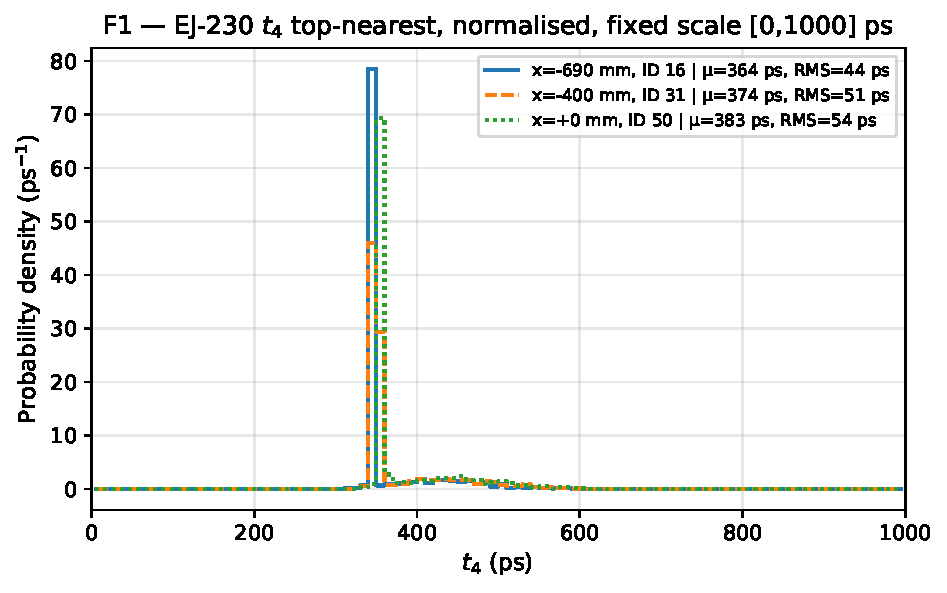
\includegraphics[height=0.48\textheight,keepaspectratio]{exec13_230_f1_t4pe_overlay_norm}
\vspace{-0.1cm}
\begin{block}{\tiny How to read this plot}
\tiny\textbf{Why:} EXEC\_12 EJ-204 histograms had auto-scale; this re-bins at 10\,ps with fixed [0,1000]\,ps range for visual comparison between runs. EJ-230 $\tau_d=1.5$\,ns (shorter than EJ-204 1.8\,ns).  \textbf{Axes:} x: $t_{4}$ arrival time (ps); y: prob. density (norm, ps$^{-1}$) or events/10\,ps (abs). Note: peak density CAN exceed 1\,ps$^{-1}$ --- correct.  \textbf{Takeaway:} Narrow (t4) or broader (t20) distribution; shape encodes scintillation + Landau fluctuations.
\end{block}

\end{frame}

\begin{frame}
\frametitle{F1 --- Overlay $t_{4}$, absolute counts [EJ-230]}
\centering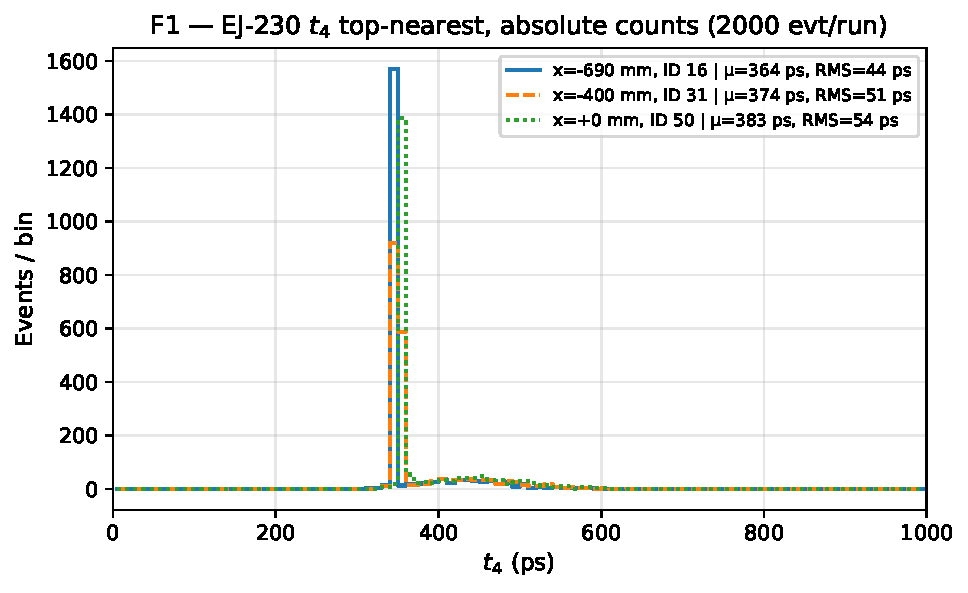
\includegraphics[height=0.48\textheight,keepaspectratio]{exec13_230_f1_t4pe_overlay_abs}
\vspace{-0.1cm}
\begin{block}{\tiny How to read this plot}
\tiny\textbf{Why:} EXEC\_12 EJ-204 histograms had auto-scale; this re-bins at 10\,ps with fixed [0,1000]\,ps range for visual comparison between runs. EJ-230 $\tau_d=1.5$\,ns (shorter than EJ-204 1.8\,ns).  \textbf{Axes:} x: $t_{4}$ arrival time (ps); y: prob. density (norm, ps$^{-1}$) or events/10\,ps (abs). Note: peak density CAN exceed 1\,ps$^{-1}$ --- correct.  \textbf{Takeaway:} Narrow (t4) or broader (t20) distribution; shape encodes scintillation + Landau fluctuations.
\end{block}

\end{frame}

\begin{frame}
\frametitle{F1 --- Individual panels $t_{4}$ (identical scale) [EJ-230]}
\centering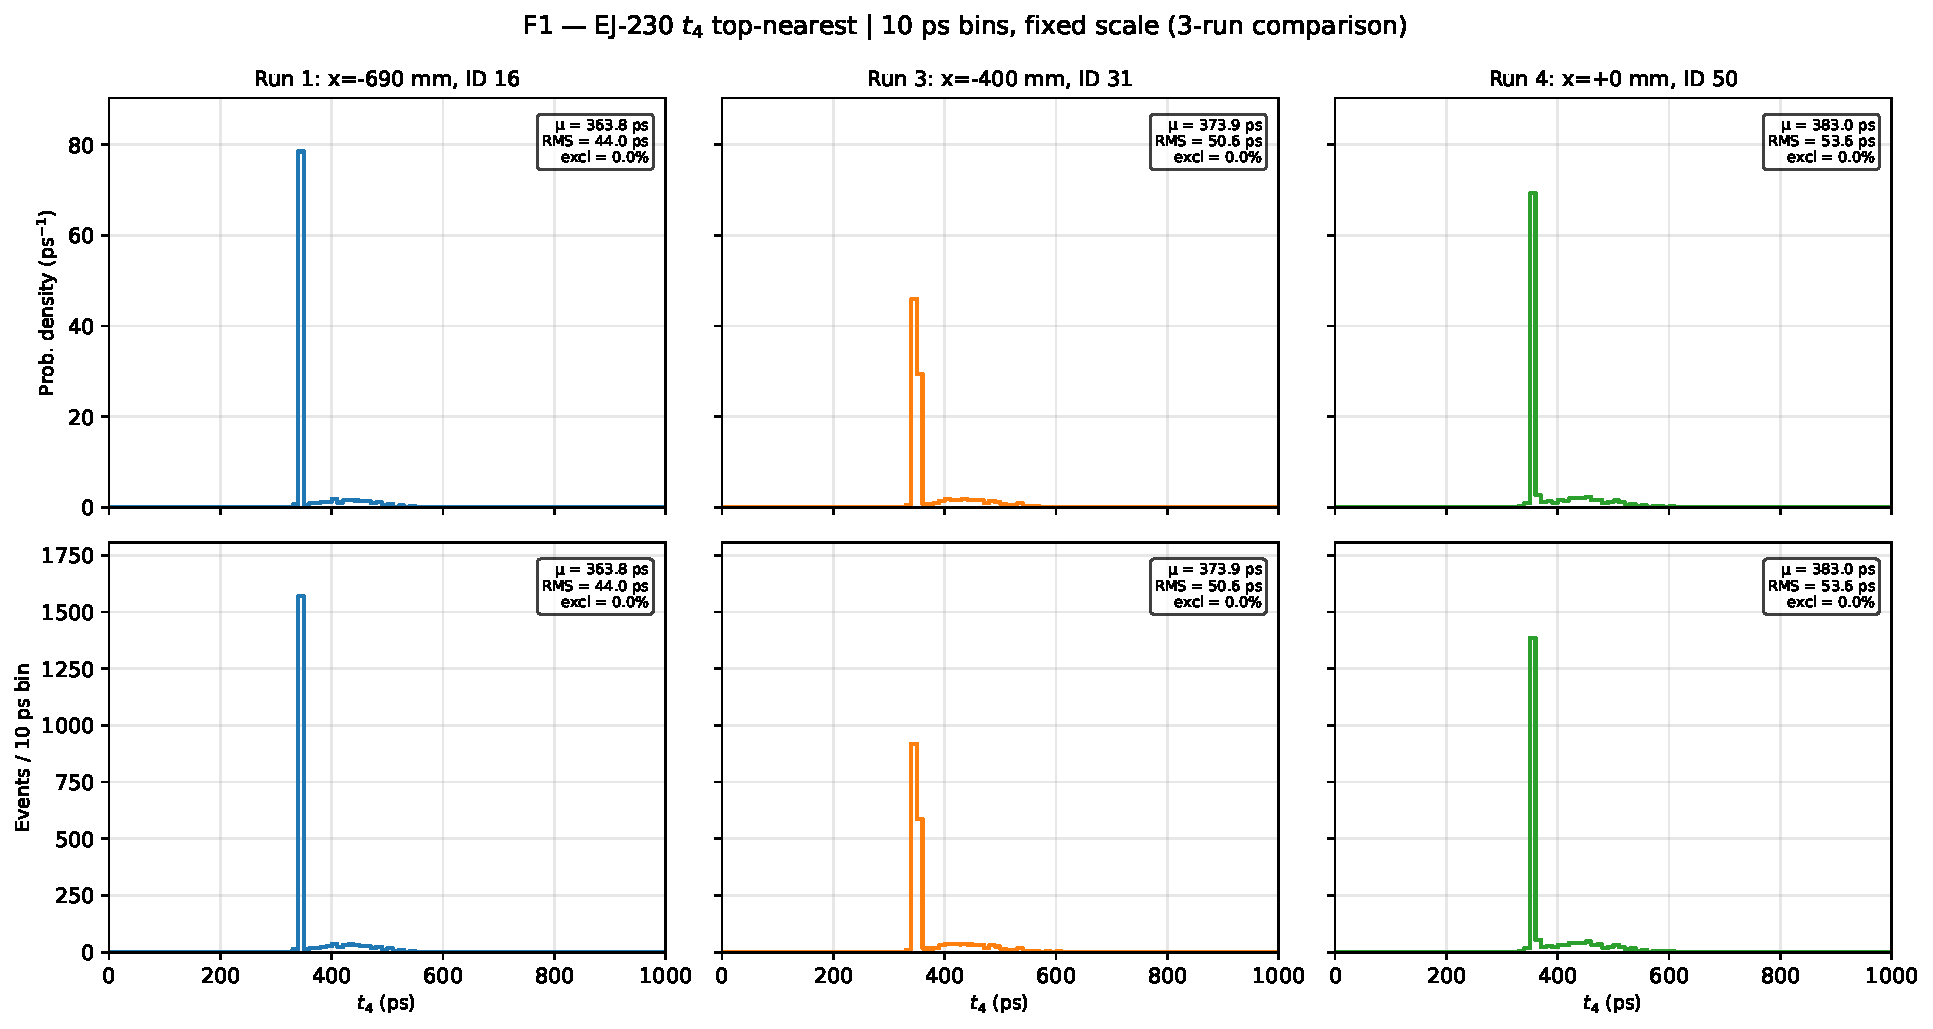
\includegraphics[height=0.52\textheight,keepaspectratio]{exec13_230_f1_t4pe_panels}
\vspace{-0.1cm}
\begin{block}{\tiny How to read this plot}
\tiny\textbf{Why:} EXEC\_12 EJ-204 histograms had auto-scale; this re-bins at 10\,ps with fixed [0,1000]\,ps range for visual comparison between runs. EJ-230 $\tau_d=1.5$\,ns (shorter than EJ-204 1.8\,ns).  \textbf{Axes:} x: $t_{4}$ arrival time (ps); y: prob. density (norm, ps$^{-1}$) or events/10\,ps (abs). Note: peak density CAN exceed 1\,ps$^{-1}$ --- correct.  \textbf{Takeaway:} Narrow (t4) or broader (t20) distribution; shape encodes scintillation + Landau fluctuations.
\end{block}

\end{frame}

\begin{frame}
\frametitle{F1 --- Overlay $t_{20}$, normalised, fixed scale [EJ-230]}
\centering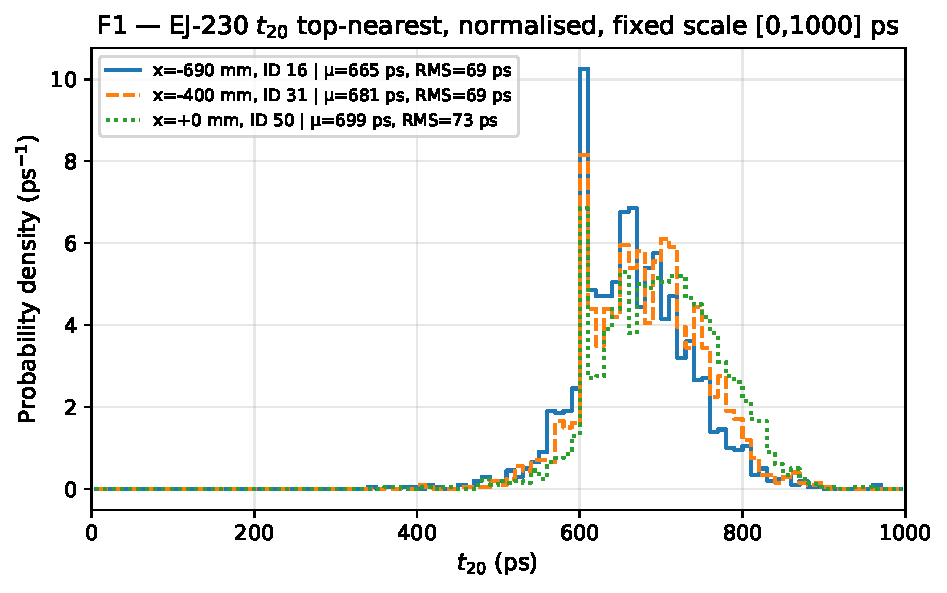
\includegraphics[height=0.48\textheight,keepaspectratio]{exec13_230_f1_t20pe_overlay_norm}
\vspace{-0.1cm}
\begin{block}{\tiny How to read this plot}
\tiny\textbf{Why:} EXEC\_12 EJ-204 histograms had auto-scale; this re-bins at 10\,ps with fixed [0,1000]\,ps range for visual comparison between runs. EJ-230 $\tau_d=1.5$\,ns (shorter than EJ-204 1.8\,ns).  \textbf{Axes:} x: $t_{20}$ arrival time (ps); y: prob. density (norm, ps$^{-1}$) or events/10\,ps (abs). Note: peak density CAN exceed 1\,ps$^{-1}$ --- correct.  \textbf{Takeaway:} Narrow (t4) or broader (t20) distribution; shape encodes scintillation + Landau fluctuations.
\end{block}

\end{frame}

\begin{frame}
\frametitle{F1 --- Overlay $t_{20}$, absolute counts [EJ-230]}
\centering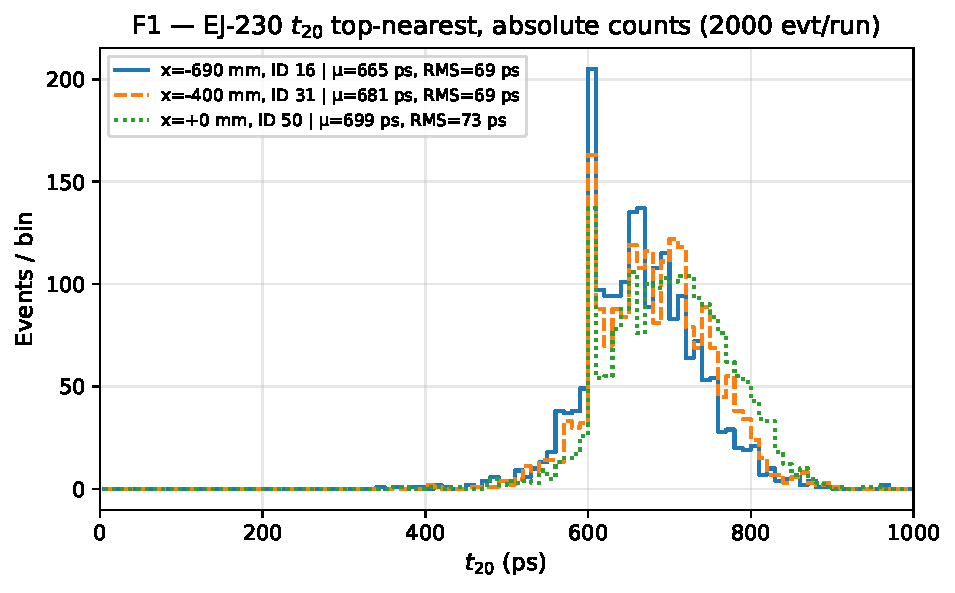
\includegraphics[height=0.48\textheight,keepaspectratio]{exec13_230_f1_t20pe_overlay_abs}
\vspace{-0.1cm}
\begin{block}{\tiny How to read this plot}
\tiny\textbf{Why:} EXEC\_12 EJ-204 histograms had auto-scale; this re-bins at 10\,ps with fixed [0,1000]\,ps range for visual comparison between runs. EJ-230 $\tau_d=1.5$\,ns (shorter than EJ-204 1.8\,ns).  \textbf{Axes:} x: $t_{20}$ arrival time (ps); y: prob. density (norm, ps$^{-1}$) or events/10\,ps (abs). Note: peak density CAN exceed 1\,ps$^{-1}$ --- correct.  \textbf{Takeaway:} Narrow (t4) or broader (t20) distribution; shape encodes scintillation + Landau fluctuations.
\end{block}

\end{frame}

\begin{frame}
\frametitle{F1 --- Individual panels $t_{20}$ (identical scale) [EJ-230]}
\centering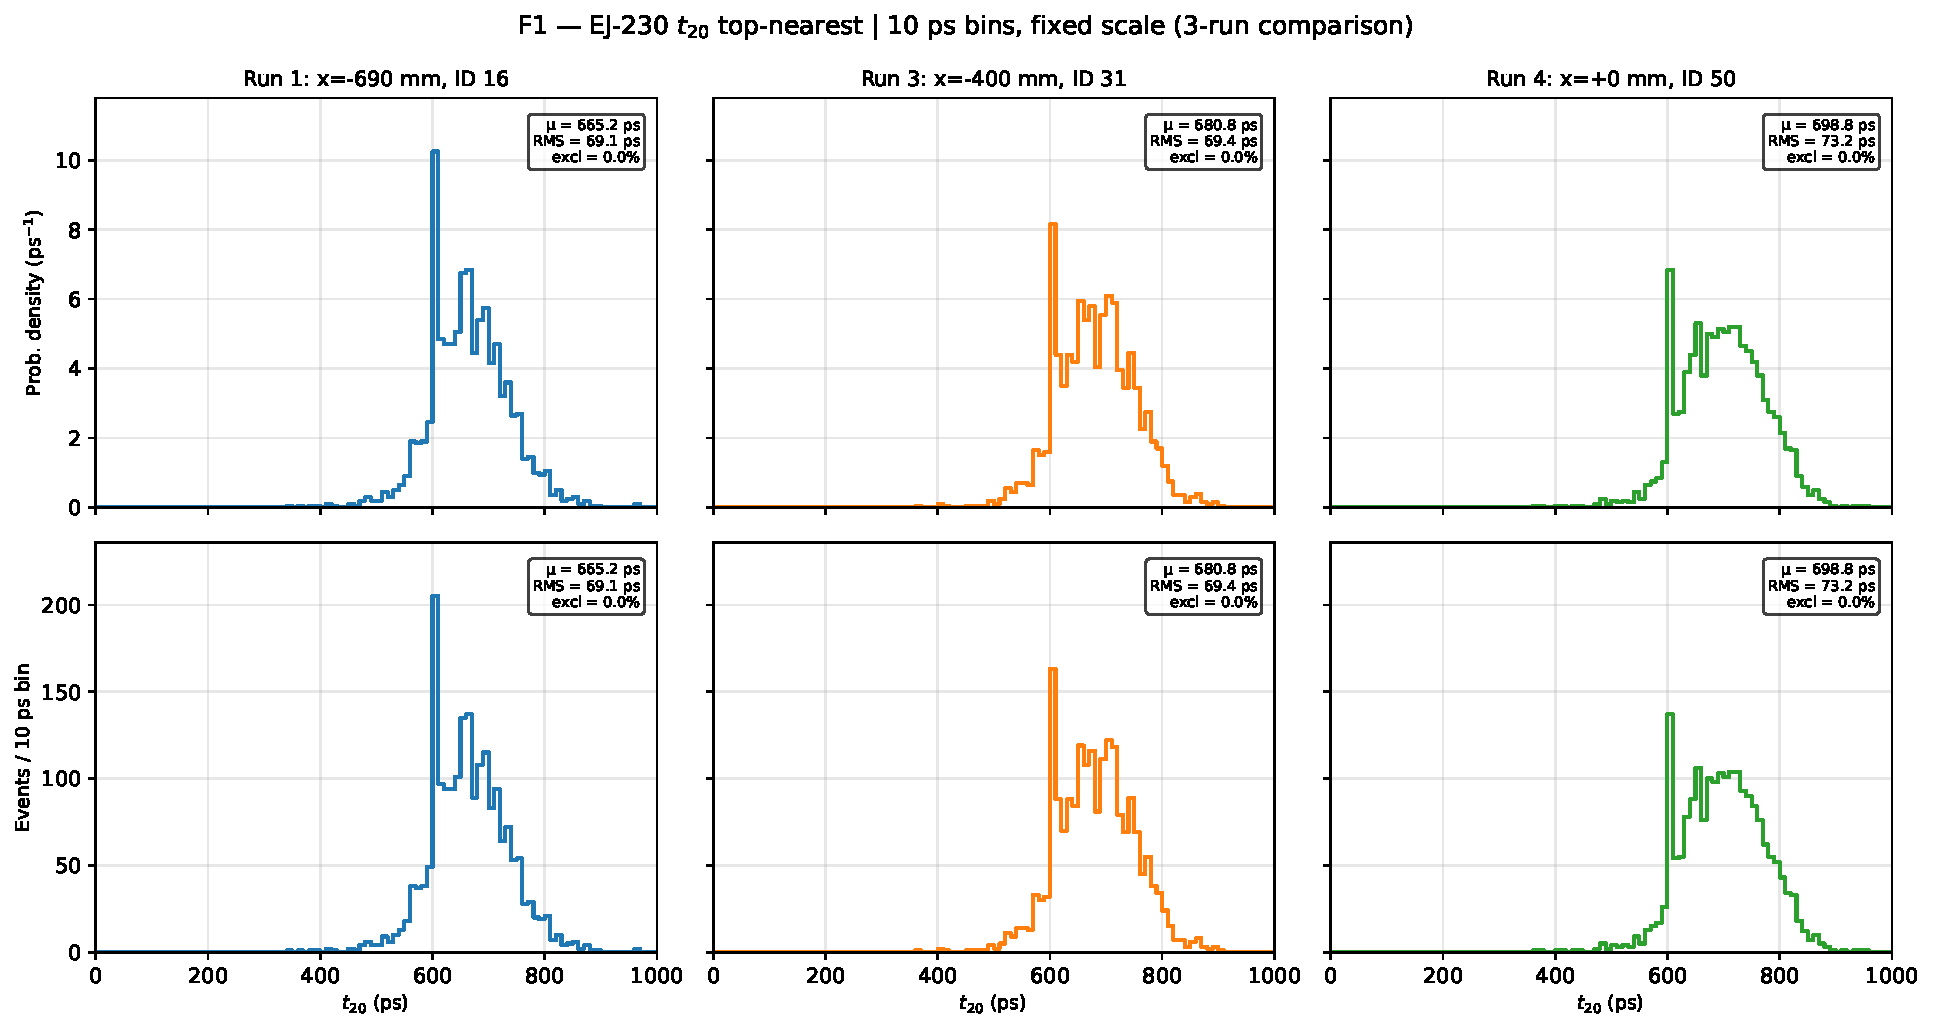
\includegraphics[height=0.52\textheight,keepaspectratio]{exec13_230_f1_t20pe_panels}
\vspace{-0.1cm}
\begin{block}{\tiny How to read this plot}
\tiny\textbf{Why:} EXEC\_12 EJ-204 histograms had auto-scale; this re-bins at 10\,ps with fixed [0,1000]\,ps range for visual comparison between runs. EJ-230 $\tau_d=1.5$\,ns (shorter than EJ-204 1.8\,ns).  \textbf{Axes:} x: $t_{20}$ arrival time (ps); y: prob. density (norm, ps$^{-1}$) or events/10\,ps (abs). Note: peak density CAN exceed 1\,ps$^{-1}$ --- correct.  \textbf{Takeaway:} Narrow (t4) or broader (t20) distribution; shape encodes scintillation + Landau fluctuations.
\end{block}

\end{frame}

\begin{frame}
\frametitle{F2 --- Run 1: $x=-690$\,mm cluster dispersion [EJ-230]}
\centering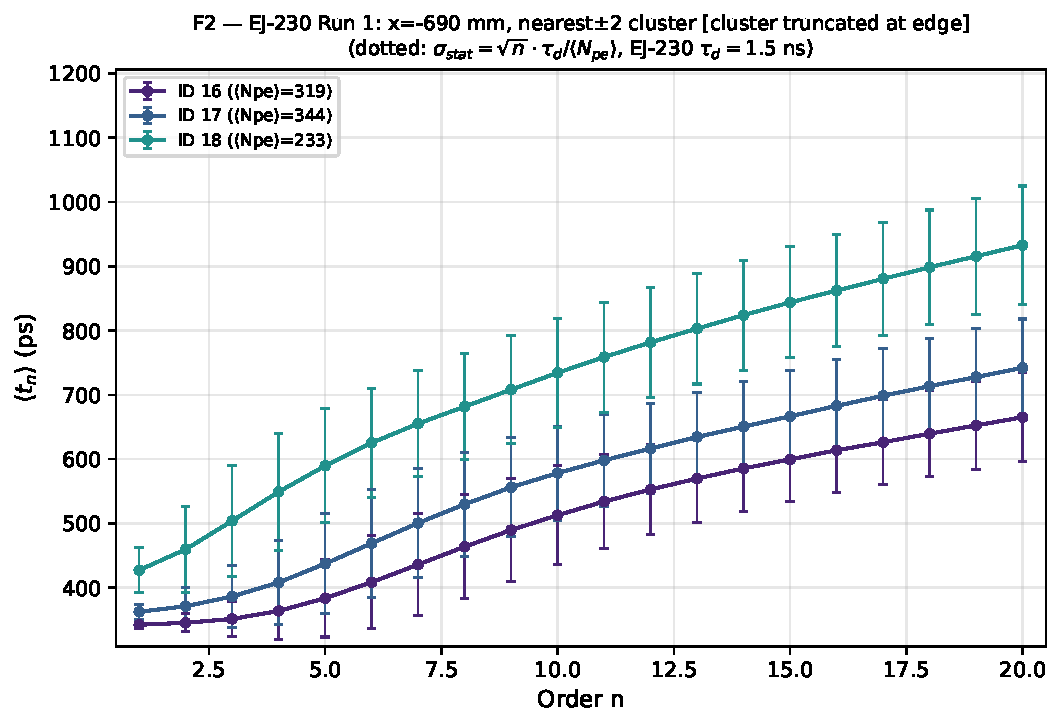
\includegraphics[height=0.50\textheight,keepaspectratio]{exec13_230_f2_cluster_-690mm}
\vspace{-0.1cm}
\begin{block}{\tiny How to read this plot}
\tiny\textbf{Why:} Do neighbour SiPMs $\pm1,\pm2$ carry the same timing as the nearest? Stat floor uses EJ-230 $\tau_d=\ejtauD$\,ns.  \textbf{Axes:} x: photon order $n$ (1--20); y: $\langle t_n\rangle$ (ps). Error bars = RMS. Dotted: stat floor $\sqrt{n}\,\tau_d/\langle N_{pe}\rangle$.  \textbf{Takeaway:} Neighbours approach stat floor when their $\langle N_{pe}\rangle$ is comparable to the nearest.
\end{block}

\end{frame}

\begin{frame}
\frametitle{F2 --- Run 3: $x=-400$\,mm cluster dispersion [EJ-230]}
\centering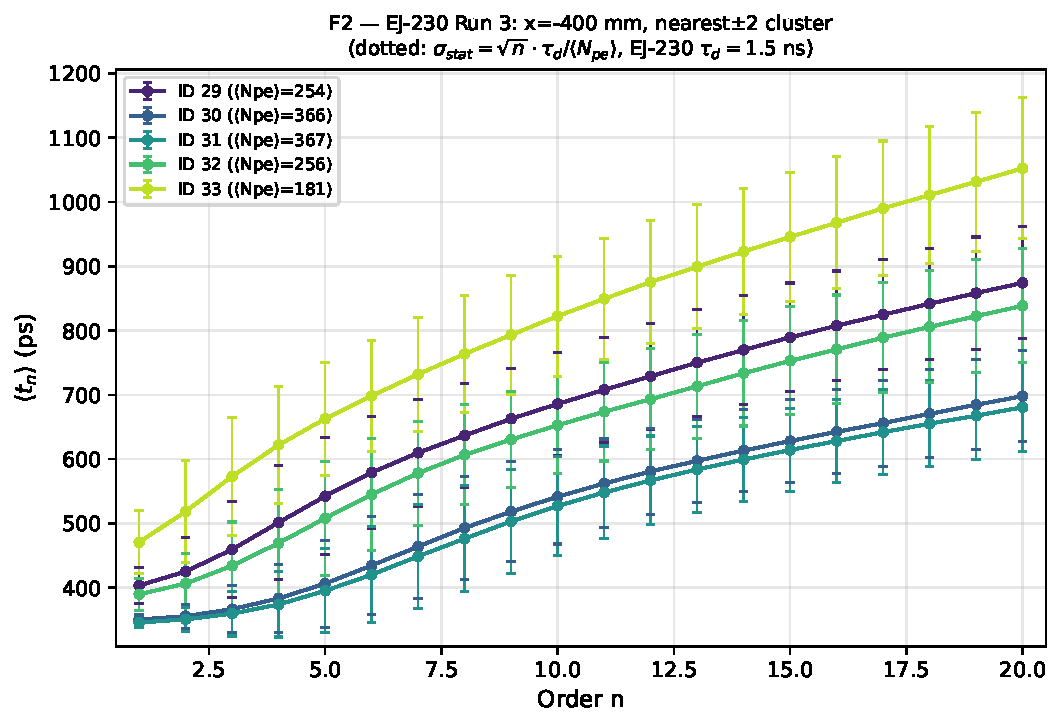
\includegraphics[height=0.50\textheight,keepaspectratio]{exec13_230_f2_cluster_-400mm}
\vspace{-0.1cm}
\begin{block}{\tiny How to read this plot}
\tiny\textbf{Why:} Do neighbour SiPMs $\pm1,\pm2$ carry the same timing as the nearest? Stat floor uses EJ-230 $\tau_d=\ejtauD$\,ns.  \textbf{Axes:} x: photon order $n$ (1--20); y: $\langle t_n\rangle$ (ps). Error bars = RMS. Dotted: stat floor $\sqrt{n}\,\tau_d/\langle N_{pe}\rangle$.  \textbf{Takeaway:} Neighbours approach stat floor when their $\langle N_{pe}\rangle$ is comparable to the nearest.
\end{block}

\end{frame}

\begin{frame}
\frametitle{F2 --- Run 4: $x=+0$\,mm cluster dispersion [EJ-230]}
\centering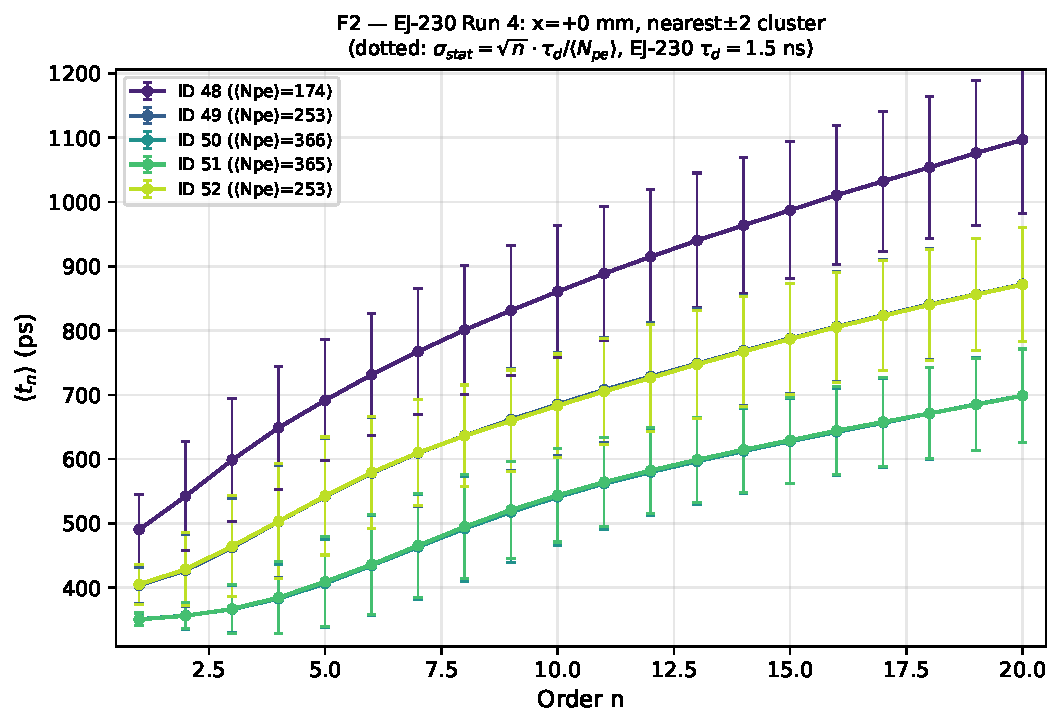
\includegraphics[height=0.50\textheight,keepaspectratio]{exec13_230_f2_cluster_+0mm}
\vspace{-0.1cm}
\begin{block}{\tiny How to read this plot}
\tiny\textbf{Why:} Do neighbour SiPMs $\pm1,\pm2$ carry the same timing as the nearest? Stat floor uses EJ-230 $\tau_d=\ejtauD$\,ns.  \textbf{Axes:} x: photon order $n$ (1--20); y: $\langle t_n\rangle$ (ps). Error bars = RMS. Dotted: stat floor $\sqrt{n}\,\tau_d/\langle N_{pe}\rangle$.  \textbf{Takeaway:} Neighbours approach stat floor when their $\langle N_{pe}\rangle$ is comparable to the nearest.
\end{block}

\end{frame}

\begin{frame}
\frametitle{F3 --- EJ-230 Top $N_{pe}$ profile (all 70 channels, fixed scale)}
\centering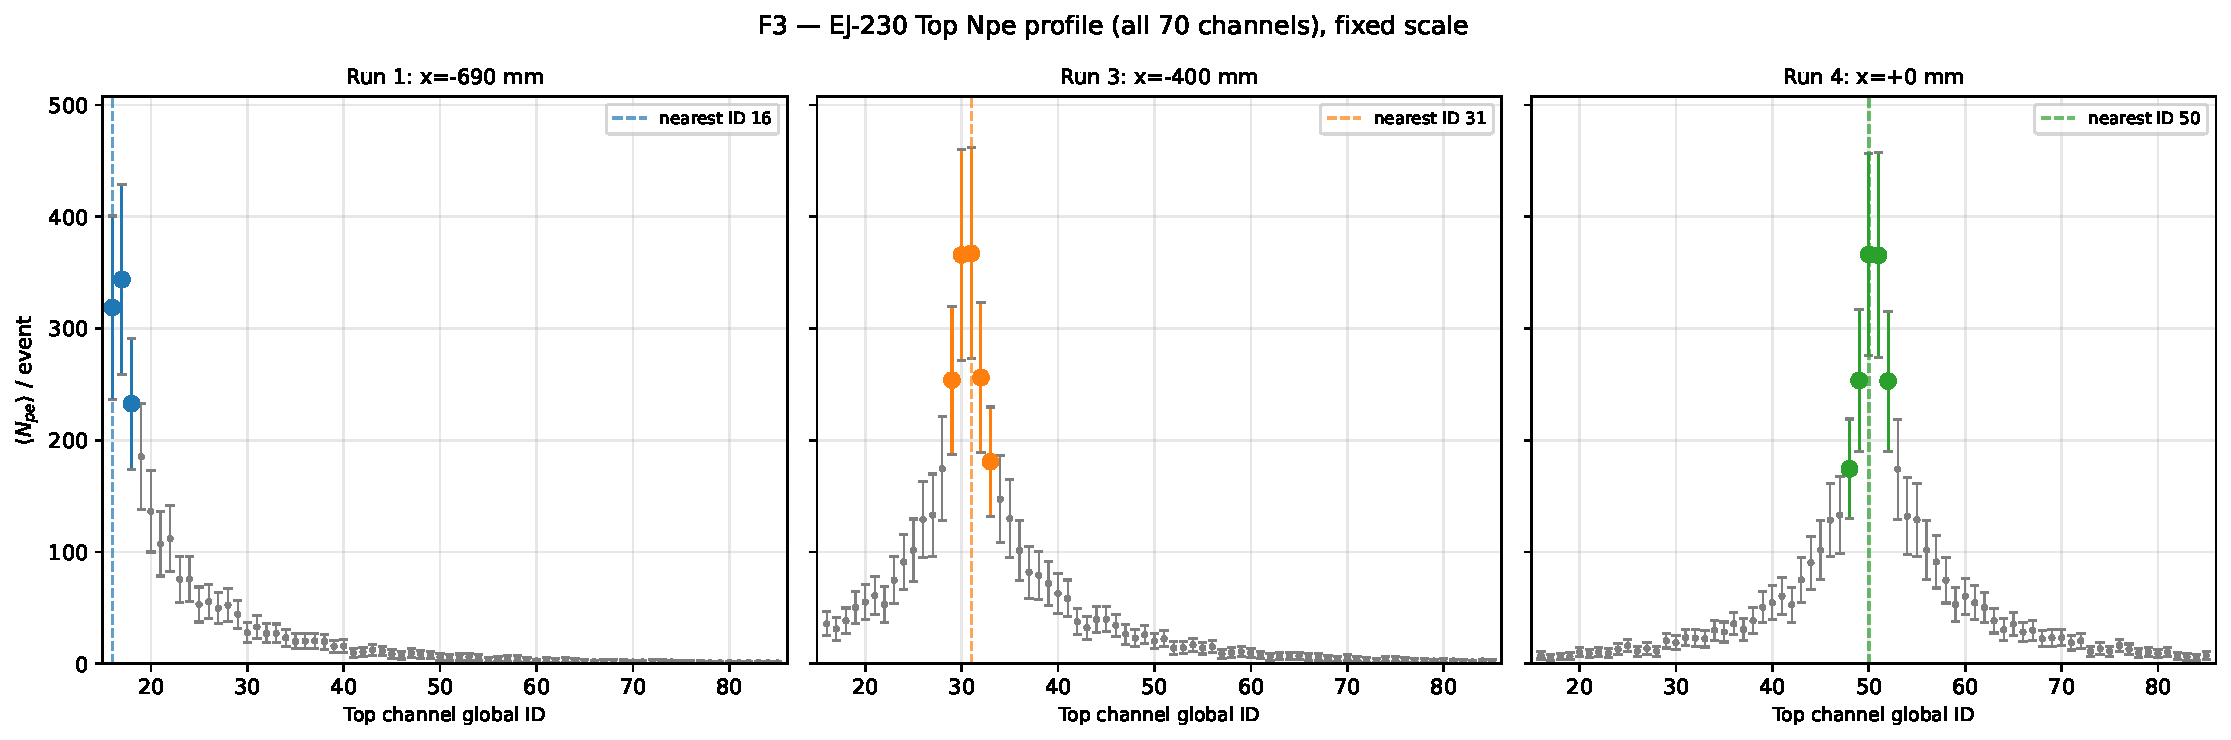
\includegraphics[width=0.98\textwidth]{exec13_230_f3_npe_profile}
\vspace{-0.1cm}
\begin{block}{\tiny How to read this plot}
\tiny\textbf{Why:} Verify nearest channel is the Npe maximum; shows photon budget across top array.  \textbf{Axes:} x: global channel ID (16--85); y: $\langle N_{pe}\rangle$/event $\pm$ RMS. Highlighted: cluster $\pm$2.  \textbf{Takeaway:} Npe falls off rapidly away from track; $\pm$2 neighbours still collect useful light.
\end{block}

\end{frame}

\begin{frame}
\frametitle{F4 --- EJ-230 timing profile $\langle t_{4}\rangle$ (eff$\geq$0.99, fixed scale)}
\centering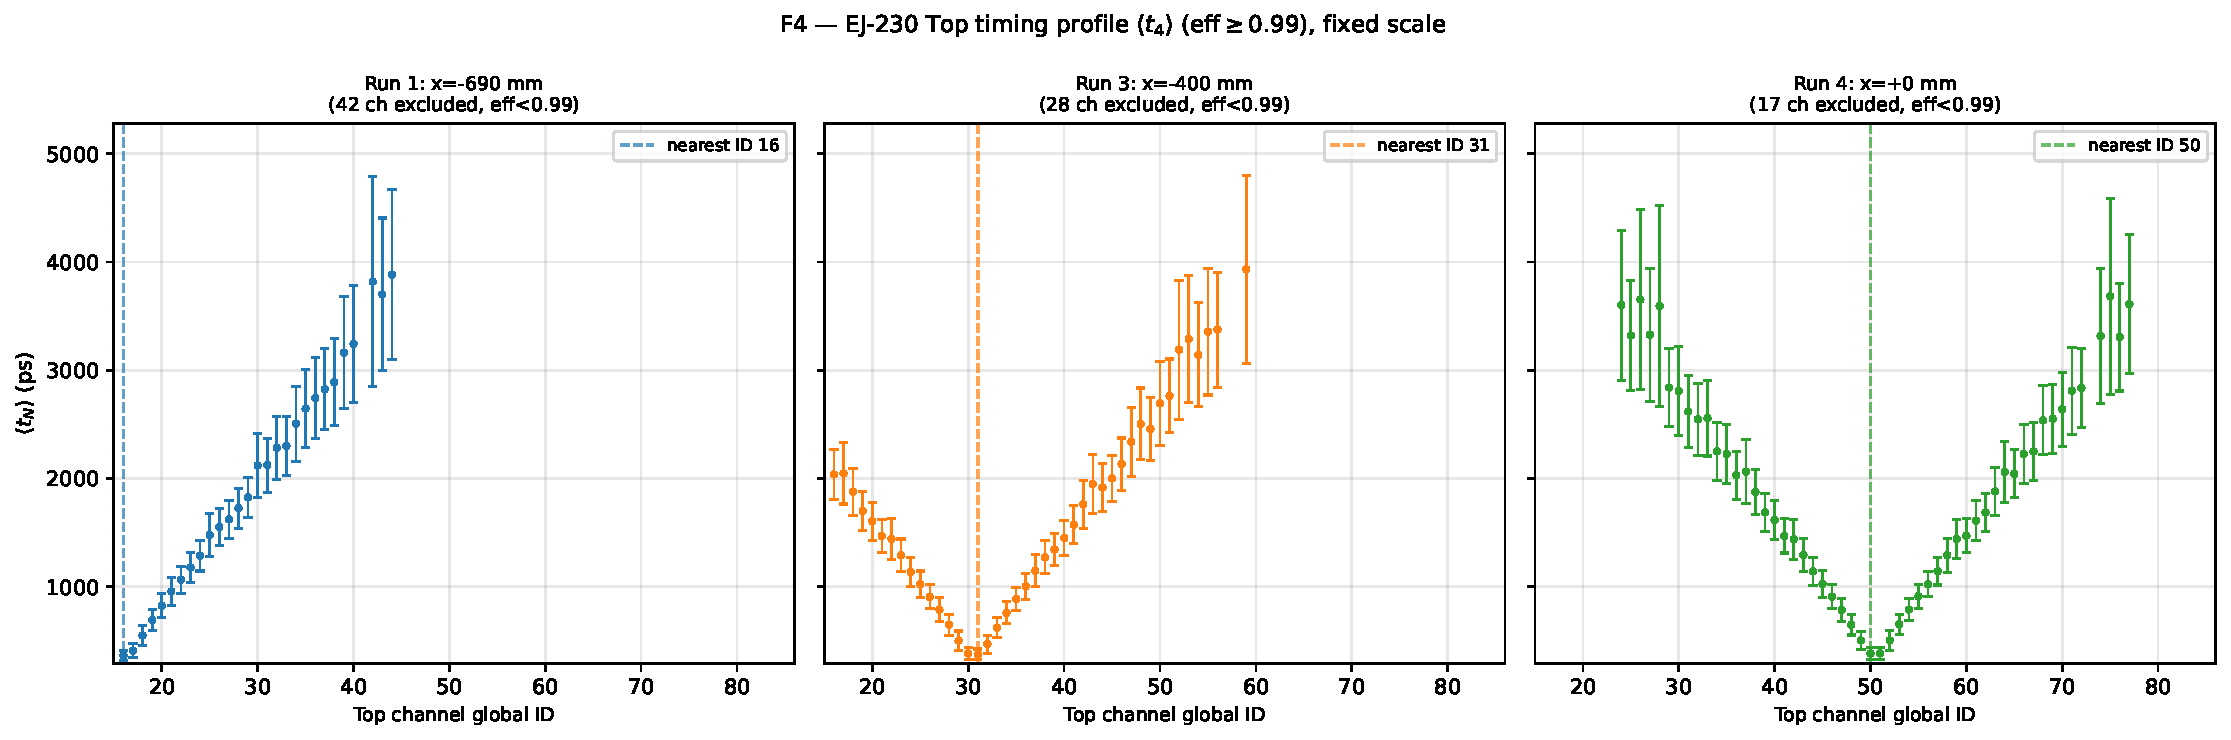
\includegraphics[width=0.98\textwidth]{exec13_230_f4_timing_t4pe}
\vspace{-0.1cm}
\begin{block}{\tiny How to read this plot}
\tiny\textbf{Why:} Only channels with eff $\geq0.99$ are shown; far channels excluded at N=20 (insufficient Npe) --- listed in CSV.  \textbf{Axes:} x: global channel ID; y: $\langle t_N\rangle$ (ps) $\pm$ RMS.  \textbf{Takeaway:} Timing rises steeply for channels far from track (longer path + lower $N_{pe}$).
\end{block}

\end{frame}

\begin{frame}
\frametitle{F4 --- EJ-230 timing profile $\langle t_{20}\rangle$ (eff$\geq$0.99, fixed scale)}
\centering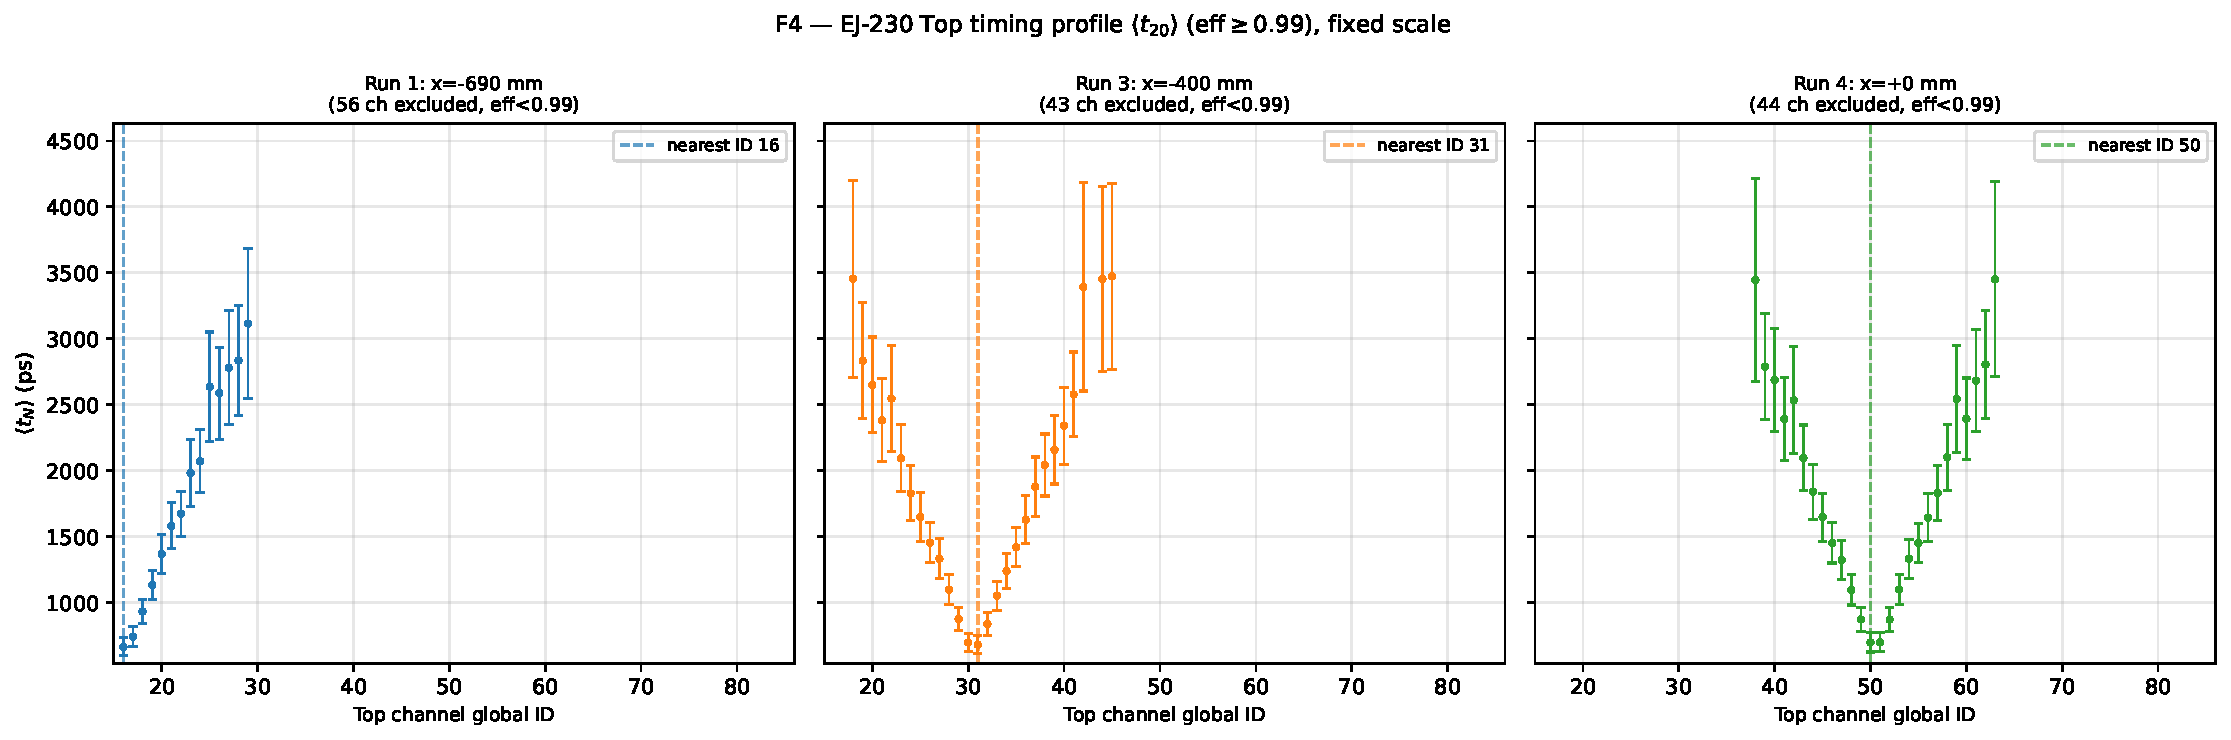
\includegraphics[width=0.98\textwidth]{exec13_230_f4_timing_t20pe}
\vspace{-0.1cm}
\begin{block}{\tiny How to read this plot}
\tiny\textbf{Why:} Only channels with eff $\geq0.99$ are shown; far channels excluded at N=20 (insufficient Npe) --- listed in CSV.  \textbf{Axes:} x: global channel ID; y: $\langle t_N\rangle$ (ps) $\pm$ RMS.  \textbf{Takeaway:} Timing rises steeply for channels far from track (longer path + lower $N_{pe}$).
\end{block}

\end{frame}

\begin{frame}
\frametitle{Validation gates [EJ-230]}
\small
\begin{itemize}
  \item \textbf{G-MAT/G-TAU}: $\tau_d=\ejtauD$\,ns (EJ-230), read from
        \texttt{analysis/exec13/common13.py} --- not a literal
  \item \textbf{G1}: nearest IDs determined programmatically from $\langle N_{pe}\rangle$
        data: $x=-690\to\text{ID }\coreRunOneNearestID$ | $x=-400\to\text{ID }\coreRunThreeNearestID$ | $x=+0\to\text{ID }\coreRunFourNearestID$
  \item \textbf{G2}: all figure panels within each family share identical axis limits
        --- verified post-plot
  \item \textbf{G3}: $n_{\rm events}=2000$ per run
  \item \textbf{G4}: $n_{\rm in}+n_{\rm excl}+n_{\rm ovfl}=2000$ per histogram
  \item \textbf{G5}: F2 x-axis labelled ``Order $n$'', range 1--20
  \item \textbf{G-MACRO}: zero \texttt{\textbackslash newcommand} with digits in the command name
\end{itemize}
\vspace{3pt}
\scriptsize All gate results: \texttt{exec13\_230\_gates.csv}.
Commit: \texttt{79e701df1a3f}.

\end{frame}

\begin{frame}
\frametitle{Provenance and methodology [EJ-230]}
\small
\textbf{Material:} EJ-230 (OPSC-106) --- $\tau_r=0.5$\,ns, $\tau_d=\ejtauD$\,ns,
yield $=\ejYield$\,ph/MeV, $\ell_{\rm att}=120$\,cm, $\lambda_{\rm peak}=391$\,nm.\\[4pt]
\textbf{Data:} 31-position beam scan, 2000 events/position.
Three positions analysed: $x=-690$, $-400$, $0$\,mm.\\[4pt]
\textbf{Algorithm:} \texttt{compute\_tN} ported unchanged from
\texttt{exec07/exec12\_tN\_analysis.py:72--100} (sorted time-to-N-th hit per event).
$t=0$: Geant4 event start (\texttt{exec07\_photon\_budget.py:342}).\\[4pt]
\textbf{No gates applied:} no SPTR, no jitter, no SPE convolution, no temporal window.\\[4pt]
\textbf{EXEC\_12-EJ230 reconciliation:} no published EXEC\_12 sigma\_fit exists for EJ-230.
EXEC\_12-style refit (25\,ps bins, mean$\pm$2RMS) computed on EJ-230 data for
informational reference only.\\[4pt]
\scriptsize Analysis script: \texttt{analysis/exec13/exec13\_230\_fixed\_scale.py}.

\end{frame}

\begin{frame}
\frametitle{F5 --- EJ-230 $t_4$ nucleus: 2\,ps bins, Gaussian fit, fixed scale}
\centering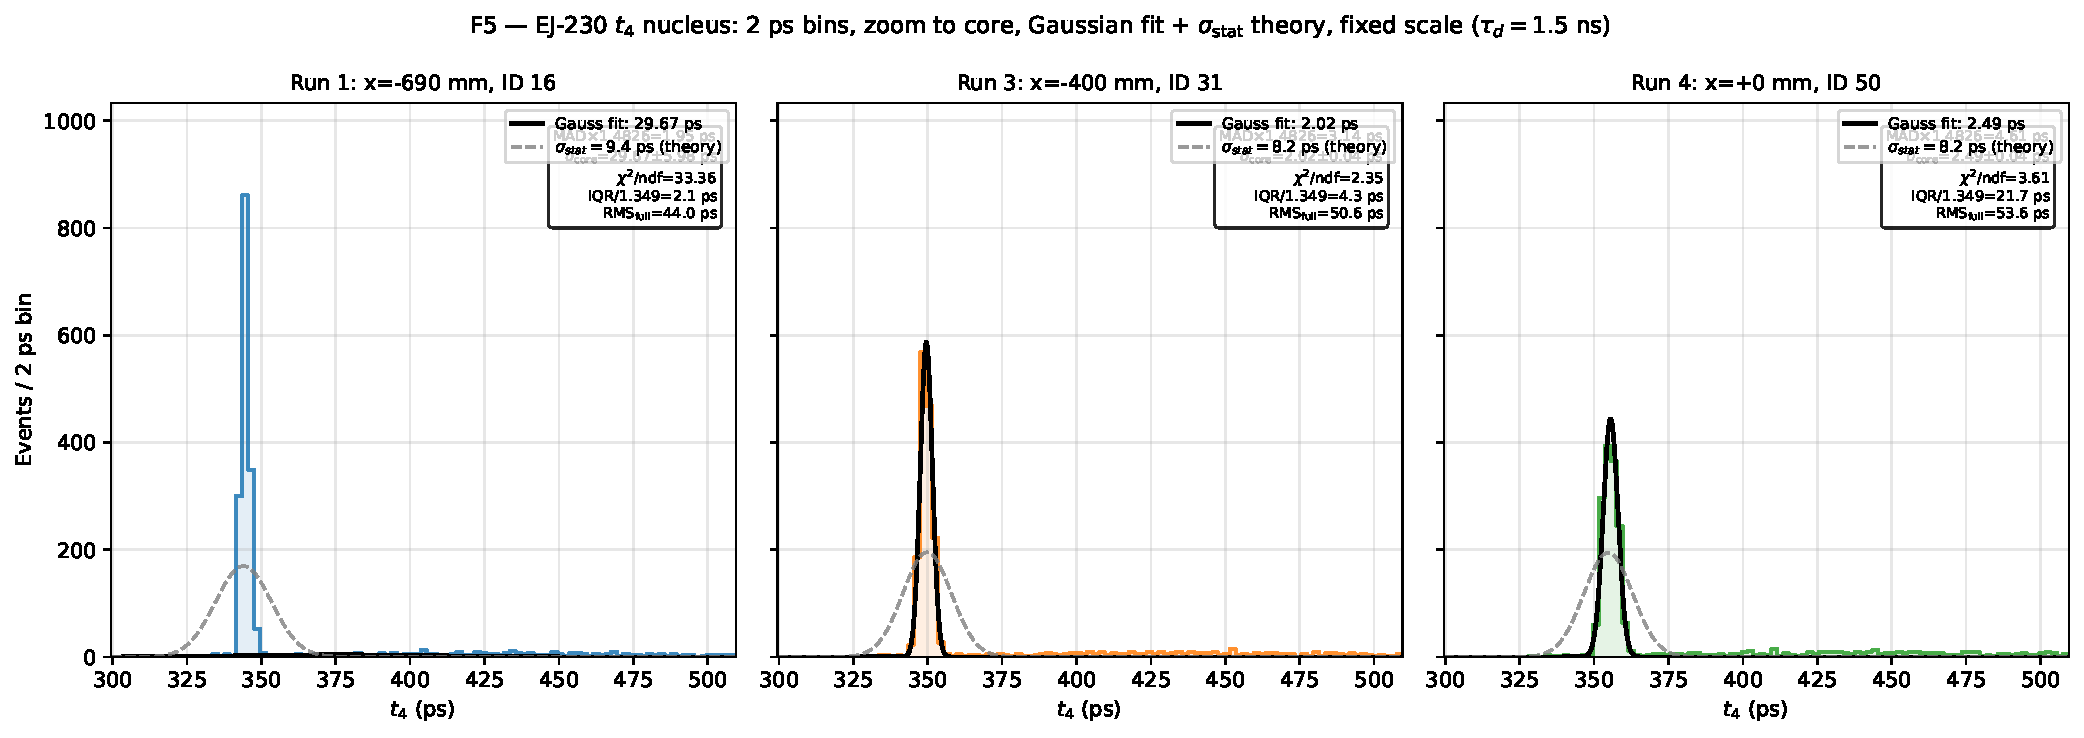
\includegraphics[width=0.98\textwidth]{exec13_230_f5_t4_core}
\vspace{-0.1cm}
\begin{block}{\tiny How to read this plot}
\tiny\textbf{Why:} RMS of $t_4$ (tens of ps) is dominated by reflection tail, not the prompt core. Zoom to mode$\pm$\coreWindowPS\,ps with 2\,ps bins to measure the narrow nucleus.  \textbf{Axes:} x: $t_4$ (ps), zoom $\approx$ mode$\pm$\coreWindowPS\,ps; y: events/2\,ps. Black solid: Gaussian fit. Gray dashed: $\sigma_{\rm stat}$ theory.  \textbf{Takeaway:} Narrow Gaussian nucleus ($\sim$ few ps); tail starts at mode$+\coreTailK\sigma_{\rm core}$.
\end{block}

\end{frame}

\begin{frame}
\frametitle{Resolución Top nearest: núcleo vs cola (EJ-230, $\tau_d=\ejtauD$\,ns)}
{\small
\begin{tabular}{lrrrrrr}
\toprule
Posición & MAD$\times$1.4826 & $\sigma_{\rm core}\pm$err & $\chi^2$/ndf
         & IQR/1.349 & RMS$_{\rm full}$ & $\sigma_{\rm stat}$ \\
         & (ps) & (ps) & & (ps) & (ps) & (ps) \\
\midrule
    $x=-690$\,mm & \coreRunOneMAD & \coreRunOneSigCore$\pm$\coreRunOneSigCoreErr & \coreRunOneChiNdf & \coreRunOneIQR & \coreRunOneRMSps & \coreRunOneSigStat \\
    $x=-400$\,mm & \coreRunThreeMAD & \coreRunThreeSigCore$\pm$\coreRunThreeSigCoreErr & \coreRunThreeChiNdf & \coreRunThreeIQR & \coreRunThreeRMSps & \coreRunThreeSigStat \\
    $x=+0$\,mm & \coreRunFourMAD & \coreRunFourSigCore$\pm$\coreRunFourSigCoreErr & \coreRunFourChiNdf & \coreRunFourIQR & \coreRunFourRMSps & \coreRunFourSigStat \\
\bottomrule
\end{tabular}}
\vspace{4pt}
\begin{alertblock}{\footnotesize Mensaje clave (aprendizaje EJ-204)}
\scriptsize
\textbf{Estimador preferido: MAD$\times$1.4826} (robusto, resistente a colas).
$\sigma_{\rm core}$ (ajuste gaussiano 2\,ps) tiende a \emph{sub-estimar} con $\chi^2$/ndf
elevado --- ver tabla.
Si IQR anómalamente grande (p.ej.\ posición central), usar MAD.
Cola = $t_4 > \mathrm{modo}+\coreTailK\sigma_{\rm core}$; dominada por reflexiones.
$\sigma_{\rm core}$ y MAD son \emph{intrínsecos de simulación} (sin SPTR, sin jitter);
la resolución real estará dominada por el SPTR ($\approx\coreSPTRps$\,ps, bloque EXEC\_02b).
\end{alertblock}

\end{frame}

\begin{frame}
\frametitle{Observaciones y próximos pasos [EJ-230]}
\small
\begin{itemize}
  \item \textbf{Material EJ-230 vs EJ-204:} $\tau_d=\ejtauD$\,ns (EJ-230) vs
        $1.8$\,ns (EJ-204) $\Rightarrow$ $\sigma_{\rm stat}(t_4)$ intrínseca menor para EJ-230.
  \item \textbf{Sin referencia EXEC\_12-EJ230:} el ajuste estilo-EXEC\_12 (25\,ps bins)
        se computa sobre datos EJ-230 como referencia informativa; no existe publicación previa.
  \item \textbf{Fuera de alcance (bloques posteriores):}
  \begin{itemize}\scriptsize
    \item Comparación lado a lado EJ-204 vs EJ-230.
    \item Introducción de SPTR/jitter (EXEC\_02b).
    \item MPPC solo en extremos; optimización de espaciado de SiPMs.
    \item Corrección de time-walk (HOOK\_WALK reservado).
  \end{itemize}
  \item \textbf{G-OVER:} revisar \texttt{exec13\_230\_report.log} para
        Overfull/Underfull --- listado en resumen final.
\end{itemize}

\end{frame}

\end{document}
